\documentclass[10pt,letterpaper]{article}
\usepackage{fullpage}
\usepackage{xcolor}
\usepackage[top=1in, bottom=1in, left=1in, right=1in]{geometry}
\usepackage{graphicx}
\usepackage{wrapfig}
\usepackage{hyperref}

\newcommand{\todo}[1]{\textcolor{red}{TODO:\ #1}}
\newcommand{\shortname}{EqMap}

\title{ECE6745 Project Proposal}
\author{Matthew Hofmann}
\date{\today}

\begin{document}

\maketitle

% Revised Sections
% Introduction
% Background (lit review)
% Baseline design

\section{Motivation}\label{sec:motivation}

As the trends of transistor scaling come to a close, the QoR (quality of
results) of EDA tools will become more of a bottleneck in the hardware design
process. Given new developments in compiler technology and automated reasoning
tools, it is possible to better study the suboptimality of the EDA tool stack.
Several of the heuristics used in core EDA algorithms were invented decades
ago, and increases in compute capacity in the modern era afford us a more
formal and exploratory approach to optimizing digital logic. In this project, I
use the automated reasoning capabilities of equality graphs (e-graphs) to more
precisely explore optimal designs points in the PPA (power, performance, area)
trade-off space. With my results, I demonstrate that e-graph driven compilers
can better span the wide gap between SAT-based, exact synthesis and fully
heuristic algorithms.

\section{Introduction}\label{sec:intro}

Over the length of this course project, I have developed a tool which uses
e-graphs to superoptimize ASIC technology mapping. Besides developing the core
optimization and mapping framework, I have developed a Verilog parser and
emitter to be able to test my technique against existing RTL tools. In short, I
will be comparing against Synopsys Design Compiler. Across 96 RTL benchmarks,
my tool, called \shortname{}, should be able to more exactly synthesize
combinational logic to standard cells. My goal is roughly 10\% area savings
without increasing the circuit depth.

I am optimistic tat my tool can outperform Synopsys on small designs, because
e-graphs can explore circuit topologies that heuristic methods cannot. However,
the real challenge may lie in the extraction algorithm. For this reason, I will
also consider optimizing for delay if that proves to be more feasible than
optimizing for area. All of these experiments were relatively low cost to
start, because I have a lot of compiler infrastructure already built up. For
instance, I have a custom, bare-bones Verilog frontend. In the following
sections, I will give the literature review needed to understand equality
graphs for superoptimization as well as ASIC technology mapping in general.

\section{Literature Review}\label{sec:background}
\subsection{E-Graphs}\label{sec:background:egraph}

Equality graphs, most commonly referred to as \textit{e-graphs}, are an
automated reasoning tool built around a union-find data
structure~\cite{eggpaper}. An e-graph is essentially a directed graph with two
extra features: (1) nodes are grouped together into \textit{e-classes} and (2)
edges always start at a node and point to an e-class. As a consequence,
e-graphs can very compactly store a collection of equivalence relations. The
prototypical example for e-graphs involves the rewriting of arithmetic
expressions. For instance, one relation conveyed in Fig.~\ref{fig:egraph} is
that \texttt{a << 1} is equal to \texttt{a * 2}. To convey equality, the
anchoring nodes \texttt{<<} and \texttt{*} are grouped in the same e-class (the
dotted box). The children of the operators are the e-classes for \texttt{a},
\texttt{2}, and \texttt{1}. It is typical that constants and variables are leaf
nodes that live in an e-class alone. However, it is important to note that the
destination of edges is always an e-class and not a node. With this
illustration, it hopefully becomes clear why e-graphs are strong at equational
reasoning. The next section will explain how we can build an optimizing
compiler out of this design.

\begin{wrapfigure}{r}{0.47\textwidth}
    \centering
    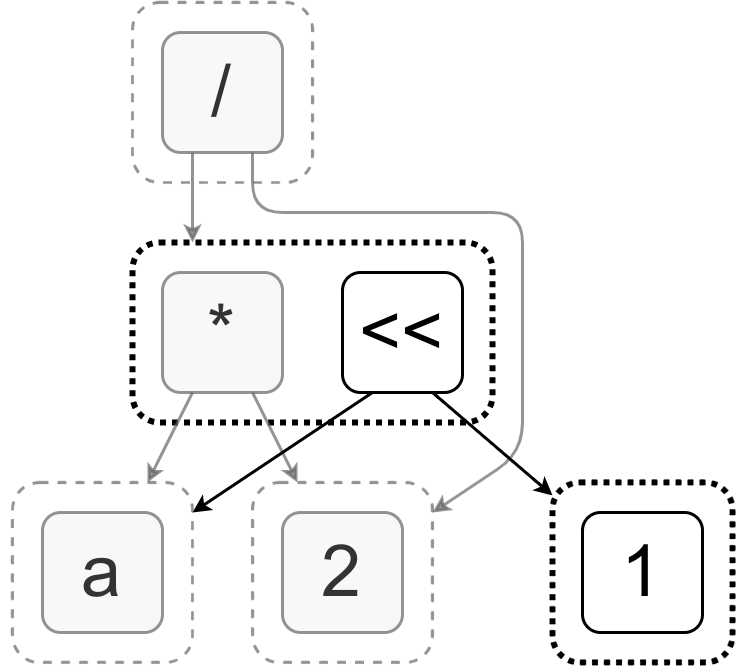
\includegraphics[width=0.44\textwidth]{img/egraph.png}
    \caption{An e-graph with 5 e-classes and 6 e-nodes.}\label{fig:egraph}
\end{wrapfigure}

E-graphs cannot reason on their own: one needs to define the notions of
equality unique to their problem domain. Continuing with the example of
computer arithmetic, we can declare arithmetic properties, like commutativity,
associativity, and distributivity, with \textit{rewrite rules}. For example,
the syntax \texttt{?a + ?b => ?b + ?a} would encode commutativity as a rewrite
rule. The left-hand side denotes a pattern to search for in the e-graph, and
the right side encodes the application of the rule. If the right-hand side of a
rule already exists in the e-graph, its e-class will be merged with the e-class
matched from the left-hand side. Otherwise, the application is inserted as a
new node in the e-class. It is important that rewrite rules are atomic. If a
rule can be broken down into multiple smaller rules, they should. This way you
can better rationalize what types of expression topologies are reachable by
your e-graph.

When using e-graphs to drive a compiler, you place your starting
expression/circuit in an empty e-graph, and each node starts alone in its
e-class. Then, you use the collection of rewrite rules to grow and build the
e-graph with alternative representations. When rewrite rules no longer
introduce new information into the graph, we say we have reach \textit{equality
    saturation}. In many cases, such as Boolean circuits, it is not possible to
fully saturated the e-graph. Instead, a time limit or size limit is reached.
Once the e-graph is built, all that is left is to extract the best rewriting of
the expression. This of course is the NP-hard part. There are several research
projects on e-graph extraction~\cite{smoothe,sparsextract}, but they are beyond
the scope of this course project. However, previous work on FPGA technology
mapping has demonstrated that fast, greedy extraction algorithms can be used
and still find area and circuit depth improvements.

In the end, e-graph driven compilers are less heuristic than conventional
compiler architectures, because they transform terms non-destructively. Typical
optimizing compilers are broken down into a pass pipeline, and the quality of
results is sensitive to the ordering of these optimization passes. Optimizing
compilers built around passes will never be able to generalize to all programs,
but in practice the results are adequate for software. In the hardware domain,
the rules of economies of scale apply and Moore's law scaling is over. Finding
an optimal design point within tight design constraints is paramount. As a
solution, e-graphs are a more formal and more optimal approach to problems in
electronic design automation. Previous work~\cite{esyn} has demonstrated the
usefulness of e-graphs for logic synthesis. Moreover, I hope to submit my own
e-graph work to ICCAD which shows 12\% area savings over vendor tools on FPGA
applications without increasing circuit depth.

\section{Baseline Compiler Design}\label{sec:baseline}

\begin{wrapfigure}{r}{0.47\textwidth}
    \centering
    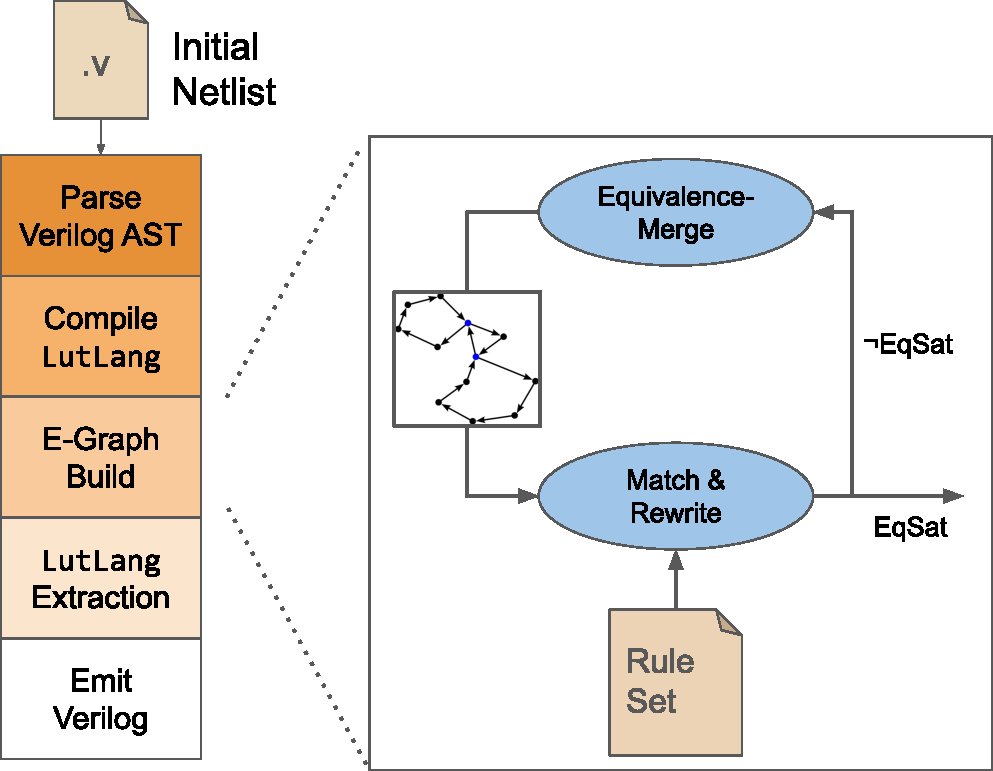
\includegraphics[width=\textwidth]{img/egraph.pdf}
    \caption{The compilation steps internal to \shortname{} Verilog tool.}\label{fig:flow:egraph}
\end{wrapfigure}

In total, I have a collection of 96 RTL benchmarks combined from three academic
sources: ISCAS'85, LGSYNTH'91, and
EPFL\footnote{\href{https://github.com/matth2k/synth-benchmarks}{https://github.com/matth2k/synth-benchmarks}}.
They are mostly combinational benchmarks, but sequential logic can also be
tested. In general, I will consider Synopsys Design Compiler as the baseline
synthesis tool.

\subsection{More Exact Synthesis}
In this experiment, I will develop logic rewriting systems and extraction
techniques that can achieve better results than Synopsys Design Compiler. In
the case of FPGA technology mapping, I already have results that show 12\% area
savings over the vendor tools without degrading timing. Moreover, I already
have a robust Boolean logic rewriting system that can be extended to standard
cell design. However, the potential pitfalls come with extraction technique.
While greedy extraction shows promise for FPGA applications, I have gut
feelings that the same extraction algorithm will not work as well for ASIC
design. ASIC cell mapping appears less like a graph covering algorithm, because
most of the cells have fanin of 1-3. FPGAs, on the other hand, have 6 input
lookup tables. Nonethless, I could be underestimating the flexibility of
standard cell design. Perhaps basic greedy extraction algorithms would still
work for synthesizing to standard cells. Moreover, I anticipate that new
e-graph extraction algorithms will improve its circuit synthesis abilities.
Although, developing new extraction algorithms is more pure compilers research
than EDA research.

\nocite{*}
\bibliographystyle{plain-annote}
\bibliography{references}

\end{document}